\pagestyle{empty}
\chapter{Generadores Minimales}
\label{cap:generadoresMinimales}
%\epigraph{I recall seeing a package to make quotes}{Snowball}

\pagestyle{headings}

\setlength{\epigraphwidth}{8.5cm}
\epigraph{\textit{Delimitaci�n..., �sta es una palabra a la que no temo, pues la labor de algo superior que posee el hombre, reside en un constante tender a limitar lo infinito, y en dividirlo y desintegrarlo en porciones perceptibles, es decir, en diferenciales.
}{\\\textit{\ \ \ \ \ \ \ \ \ \ \ \ \ \ \ \ \ \ \ \ \ \ \ \ \ \ \ \ \ \ \ \ \ \ \ \ \ \ \ \ \ \ \ \ \ \ \ \ \ \ \ \ \ \ \ \ \ \ \ \ \ \ Nosotros}\\\textup{\ \ \ \ \ \ \ \ \ \ \ \ \ \ \ \ \ \ \ \ \ \ \ \ \ \ \ \ \ \ \ \ \ \ \ \ \ \ \ \ \ \ \ \ \ \ \ \ \ \ \ \ \ \ \ \ \ \ \ \ \ \ Y. Zamiatin}}
}


\begin{table*}[htbp]
\caption*{}
%\label{tabla:ejemploPeliculas}
\centering
%{\scriptsize
\begin{tabular}{p{4.0cm}p{7.0cm}}
 \hline
 T�tulo: & Minimal generators, an affordable approach by means of massive computation\\
 Autores: & Fernando Benito-Picazo, Pablo Cordero, Manuel Enciso, �ngel Mora\\
 Revista: & The Journal of Supercomputing, Springer\\
 Factor Impacto JCR: & 1,532. Posici�n 44 de 103 (Q2)\\
 A�o: & 2017\\
 Categor�a: & Computer Science, Theory \& Methods\\
 Publicaci�n: & 4 junio 2018\\
 DOI: & 10.1007/s11227-018-2453-z\\
 \hline
\end{tabular}
%}
\end{table*}

\clearemptydoublepage

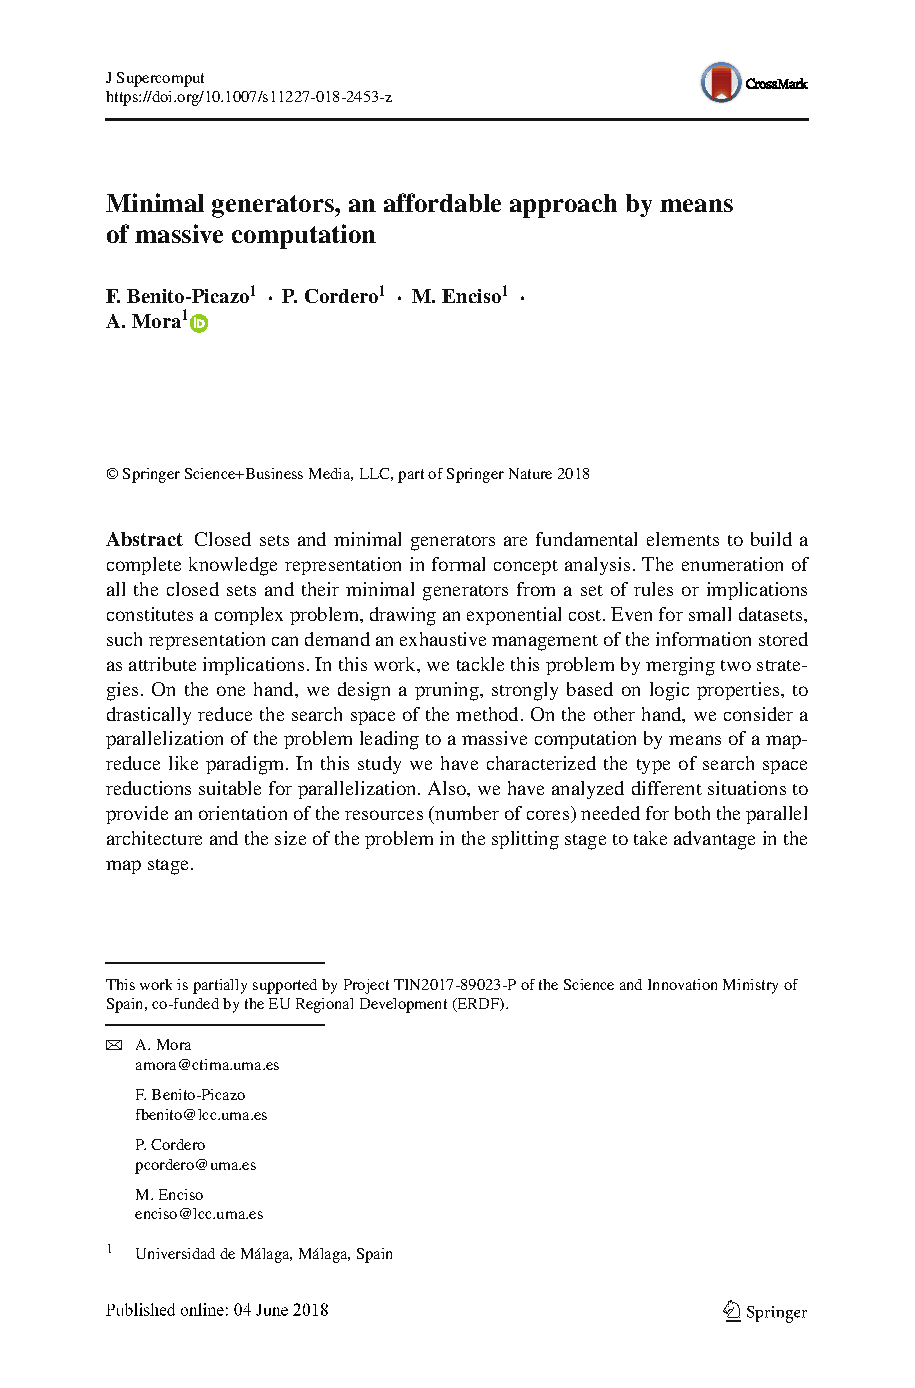
\includepdf[pages=-,scale=.9,pagecommand={}]{paperGeneradoresMinimales.pdf}

